\documentclass[11 pt]{article}
\usepackage{subcaption}
\usepackage{amsmath,amsfonts,parskip}
\usepackage[a4paper]{geometry}
\usepackage[T1]{fontenc}
\usepackage{enumerate}
\usepackage{graphicx}
\usepackage{cleveref}

\begin{document}

\begin{center}
       \large{
       \textbf{Computational Physics - PH3264} \break
       Module 4 - Partial Differential Equations
}
\end{center}
\textbf{Krishna Iyer V S \hfill Roll:20201017}
\hrule 
\vspace{0.3cm}

\begin{enumerate}
\item
The question boils down to 1-D lattice/rod with fixed temperatures at both ends. Recasting the problem and solving it analytically, we obtain T(20,20)$=1.8$ K. The value at (20,20) obtained computationally is 1.78996.
 The value The heatmap and the 3-D plot have been shown in Figure \ref{q1_heatmap} and \ref{q1_3dplot} respectively.
\begin{figure*}[ht!]
\centering
\begin{subfigure}{0.5\textwidth}
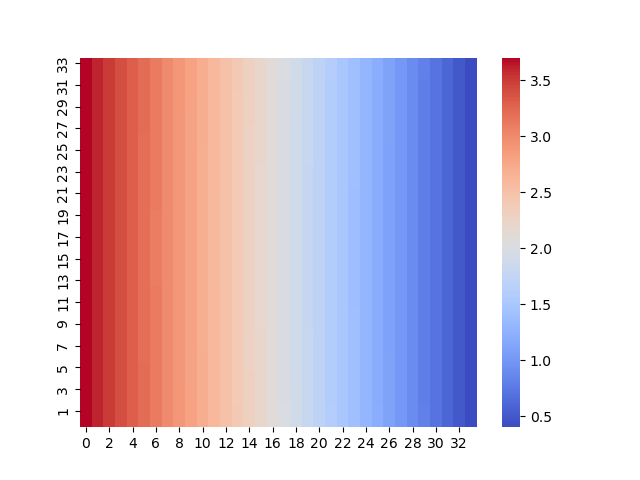
\includegraphics[width=2.5in]{../figures/Q1-heatmap.png}
\caption{Heatmap Q1}
\label{q1_heatmap}
\end{subfigure}%
~
\begin{subfigure}{0.5\textwidth}
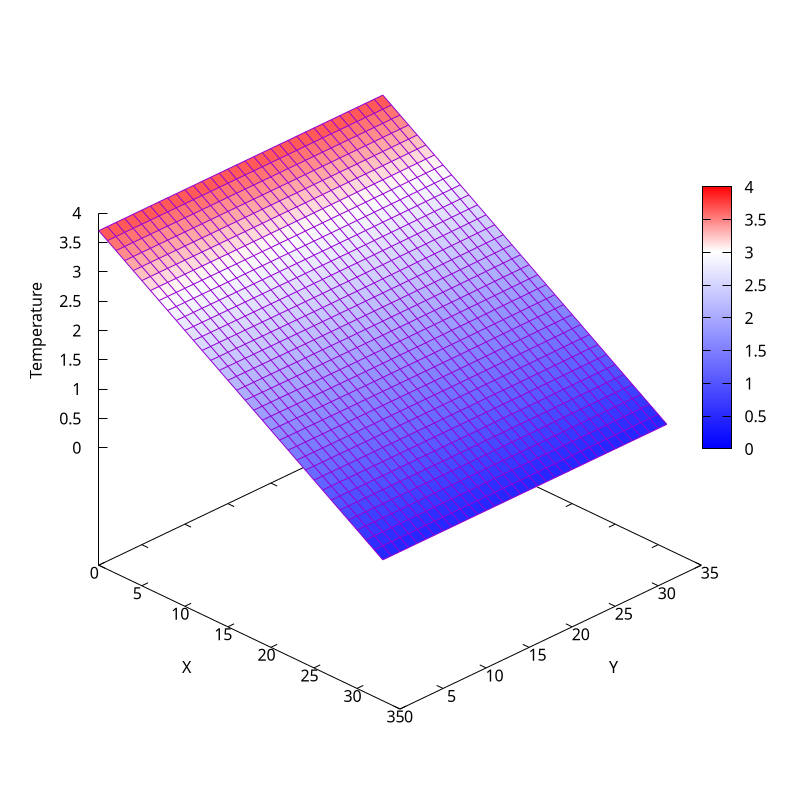
\includegraphics[width=2.5in]{../figures/Q1-3d.png}
\caption{3-D Plot for Q1}
\label{q1_3dplot}
\end{subfigure}
\end{figure*}

\item The value of the function at (20,20) is 1550 K.
\begin{figure*}[ht!]
\centering
\begin{subfigure}{0.5\textwidth}
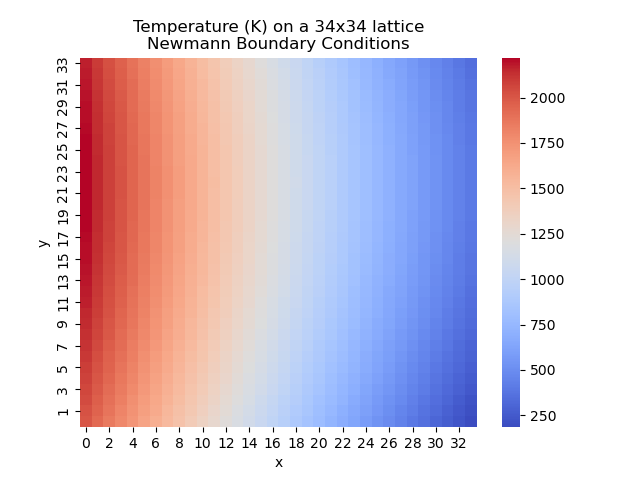
\includegraphics[width=2.5in]{../figures/Q2-heatmap.png}
\caption{Heatmap Q2}
\label{q2_heatmap}
\end{subfigure}%
~
\begin{subfigure}{0.5\textwidth}
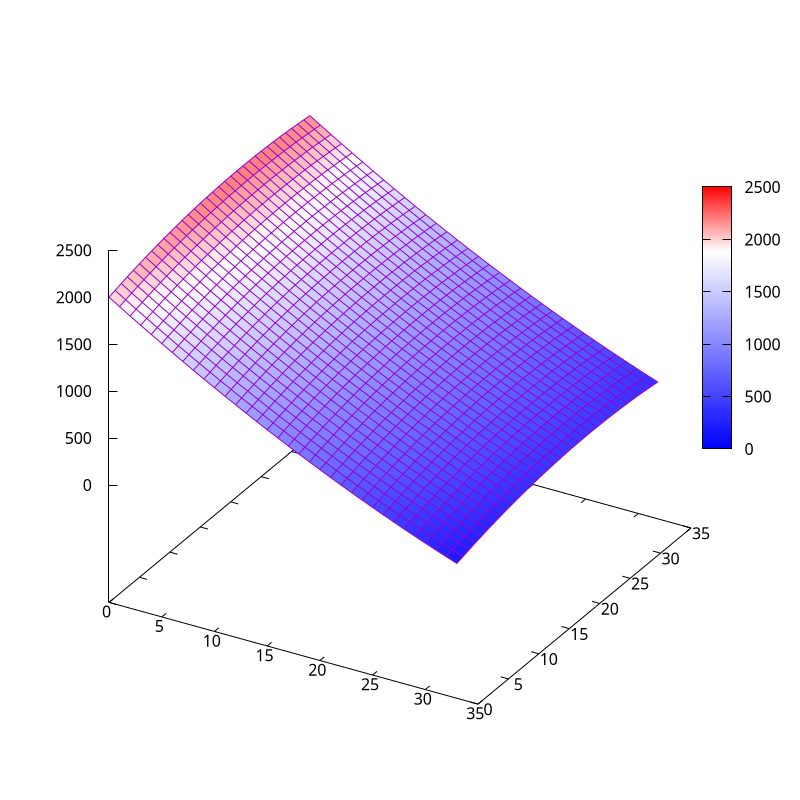
\includegraphics[width=2.5in]{../figures/Q2-3d.png}
\caption{Heatmap Q2}
\label{q2_3dplot}
\end{subfigure}
\end{figure*}
\end{enumerate}
\end{document}
